\documentclass{article}
\usepackage[margin=1in]{geometry}
\usepackage{tikz}
\usepackage{amsmath}
\pagestyle{empty}

\begin{document}
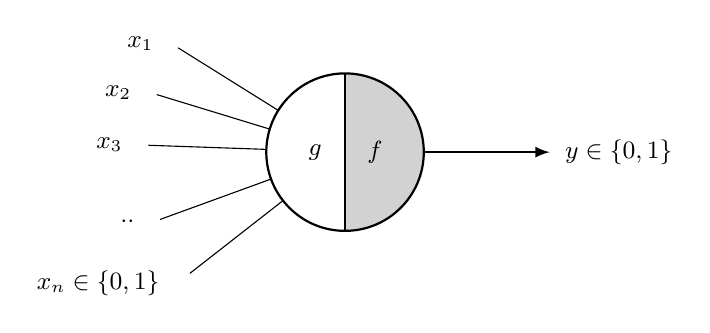
\begin{tikzpicture}[>=latex, font=\small]

  \def\R{1.0}

  % Shaded right half (function f)
  \fill[gray!35] (0,0) -- (0,\R)
    arc[start angle=90, end angle=-90, radius=\R] -- cycle;

  % Full circle
  \draw[thick] (0,0) circle (\R);

  % Vertical divider
  \draw[thick] (0,-\R) -- (0,\R);

  % Labels g and f
  \node at (-0.38, 0) {$g$};
  \node at ( 0.38, 0) {$f$};

  % x1 at ~148 degrees
  \draw[thin] ({cos(148)*2.5},{sin(148)*2.5}) -- ({cos(148)*1.0},{sin(148)*1.0});
  \node[left=3pt] at ({cos(148)*2.6},{sin(148)*2.6}) {$x_1$};

  % x2 at ~163 degrees
  \draw[thin] ({cos(163)*2.5},{sin(163)*2.5}) -- ({cos(163)*1.0},{sin(163)*1.0});
  \node[left=3pt] at ({cos(163)*2.6},{sin(163)*2.6}) {$x_2$};

  % x3 at ~178 degrees
  \draw[thin] ({cos(178)*2.5},{sin(178)*2.5}) -- ({cos(178)*1.0},{sin(178)*1.0});
  \node[left=3pt] at ({cos(178)*2.6},{sin(178)*2.6}) {$x_3$};

  % dots at ~200 degrees
  \draw[thin] ({cos(200)*2.5},{sin(200)*2.5}) -- ({cos(200)*1.0},{sin(200)*1.0});
  \node[left=3pt] at ({cos(200)*2.6},{sin(200)*2.6}) {$\cdot\cdot$};

  % xn at ~218 degrees
  \draw[thin] ({cos(218)*2.5},{sin(218)*2.5}) -- ({cos(218)*1.0},{sin(218)*1.0});
  \node[left=3pt] at ({cos(218)*2.7},{sin(218)*2.7}) {$x_n \in \{0,1\}$};

  % Output arrow
  \draw[->, thick] (1.0, 0) -- (2.6, 0);
  \node[right=2pt] at (2.6, 0) {$y \in \{0,1\}$};

\end{tikzpicture}
\end{document}
